% ----------------------------------------------------------------------------------------------------- %
% Capítulo 5 - METODOLOGIA
% ----------------------------------------------------------------------------------------------------- %
\chapter{Metodologia Proposta}
\label{cap:metodologia}

\noindent No decorrer deste capítulo é descrito a aplicação das técnicas para avaliação do aprendizado dos acadêmicos da turma de Álgebra Linear do curso de Ciência da Computação da Universidade Federal do Tocantins, bem como também a Engenharia de \textit{Software} abordada no Capítulo 3 (Fundamentação Teórica) e os recursos aplicados para o desenvolvimento do \textit{software}. O objetivo desse é demonstrar as metodologias adotadas para a avaliação do aprendizado do alunos e englobando o desenvolvimento das funcionalidades do \textit{software} AlfaGebra. 

A estrutura desta capítulo está dividido em duas seções principais, sendo elas: Avaliação do aprendizado e desenvolvimento da plataforma, e nelas estão incluídos subseções que são de grande importância para o entendimento do funcionamento.

\section{Avaliação do aprendizado}
\noindent A presente pesquisa objetiva avaliar o aprendizado dos acadêmicos a partir da utilização da plataforma de ensino e aprendizagem AlfaGebra, e para esse fim, está sendo estudada a turma do período 2017-1, turma essa que não utilizará o \textit{software} AlfaGebra no decorrer do período e será também estudada a turma do período 2017-2, a qual utilizará \textit{software} no decorrer do período. Entre ambas as turmas será comparado o nível de aprendizado com o sistema, para que assim possa ser estabelecido se houve melhora no aprendizado da turma que utilizou a ferramenta ou não. É importante salientar que para as duas turmas o professor ministrante será o mesmo, tornando por conseguinte um ponto de grande importância, pois a metodologia aplicada no decorrer da turma que não utilizará o \textit{software} será a mesma com a que utilizará a ferramenta, destacando o ponto que diferencia só no quesito de utilização do sistema.

Para a metodologia de avaliação do desempenho dos acadêmicos será aplicado a pesquisa-ação, que é um método de pesquisa em campo, ao qual os dados são coletados no local em que ocorrer o problema, por meio de questionários e/ou entrevistas, mas a presente pesquisa em questão abordará a aplicação de questionários. Um ponto de destaque nessa metodologia é que ela trata de um estudo de forma qualitativa e quantitativa, pois o objetivo da avaliação é verificar melhora no aprendizado dos estudantes, pois nas etapas inciais foi realizado um estudo nos três últimos semestre a fim de identificar o quantitativo de alunos reprovados por faltas, aprovados por notas e reprovados por notas.

Para a realização desse objetivo será aplicado o método de avaliação dos acadêmicos através de coletas de dados e como instrumentos de geração de dados serão aplicados questionários de acordo com as especificações descritas a seguir:

\begin{enumerate}
    \item Questionário base - nessa etapa foi aplicado um questionário base com perguntas objetivas de múltipas escolhas e discursivas com foco em identificar o perfil dos estudantes, tais como a quantidade de vezes que o estudante está realizando a disciplina, os métodos que são aplicados para o aprendizado dos conteúdos abordados na disciplina, dificuldade encontrada na disciplina, se a aplicação de recursos tecnológicos facilitaria o aprendizado, entre outras questões relevantes, vide Apêndice \ref{questionario_base} II. Importante ressaltar que esse questionário foi aplicado junto a turma de Álgebra Linear que não está utilizando o \textit{software} como ferramenta de aprendizagem.
    
    \item Questionário avaliação - na presente etapa será aplicado um questionário com objetivo de identificar a melhora no aprendizado dos acadêmicos, com perguntas semelhantes a etapa anterior, tais como: a partir da utilização da plataforma houve melhora no seu aprendizado, como seria seu aprendizado sem a plataforma, entre outras perguntas. É importante destacar que o questionário será aplicado junto a turma de Álgebra Linear que estará utilizando a plataforma AlfaGebra como recursos tecnológicos para o aprendizado e nessa etapa, periodicamente, os pesquisadores estarão acompanhando os estudantes a fim de identificar pontos chaves no aprendizado.
\end{enumerate}


\section{Desenvolvimento da Plataforma}
\noindent Para o desenvolvimento da plataforma AlfaGebra algumas etapas estão sendo aplicadas para a conclusão do sistema. Inicialmente, foi desenvolvido o documento de especificações de requisitos, vide Apêndice \ref{apendice_especificacao_requisitos} I, ao qual de acordo com Sommerville \cite{2013:Sommerville} esse documento abrange as características do sistema, tais como o que o sistema deve fazer, as propriedades emergentes desejáveis e essenciais e as restrições quanto à operação do sistema e quanto aos processos de desenvolvimento de \textit{software}. 

Após, será realizado a prototipagem das telas, a fim de criar os esboços das telas que oferecerão suporte para o desenvolvimento do sistema. Em seguida, serão criados os diagramas de UML (\textit{Unified Modeling Language}) do sistema, que define uma série de artefatos que ajudam na tarefa de modelar e documentar o sistema orientado a objeto que será desenvolvido.

Com as etapas supracitadas concluídas, será iniciado o desenvolvimento do código fonte do \textit{software} e com a conclusão do sistema será realizado o teste de usabilidade, com objetivo de verificar junto aos usuários a facilidade que o \textit{software} apresenta ao usar. É importante enfatizar que no decorrer do desenvolvimento do sistema estarão ocorrendo testes de funcionalidades, isso nos módulos já concluídos a fim de encontrar falhas e serem corrigidas.

\subsection{Conteúdos trabalhos no \textit{software}}
\noindent Nesta seção estão descritos os conteúdos que irão ser abordados no \textit{software}, tanto para sistemas de equações lineares como espaço vetorial. Todo o conteúdo abordado segue o plano de ensino da disciplina de Álgebra Linear do curso de Ciência da Computação.  

\subsubsection{Sistemas de equações lineares:}
\begin{itemize}
    \item[1)] Operações elementares
    \item[2)] Matriz forma escada ou linha reduzida
    \item[3)] Teorema sistema de equações lineares
    \item[4)] Soluções de Sistema de n equações lineares com m variáveis
\end{itemize}

\subsubsection{Espaço Vetorial:} 
\begin{itemize}
    \item[1)] Espaços Vetoriais
    \item[2)] Propriedades dos espaços vetoriais
    \item[3)] Subespaços vetoriais
    \item[4)] Combinação linear
    \item[5)] Subespaço gerado
    \item[6)] Dependência e Independência Linear
    \item[7)] Base de um espaço vetorial
    \item[8)] Matriz de mudança de base
\end{itemize}

A plataforma apresentará material teórico sobre cada tópicos e exercícios resolvidos para que o acadêmicos possam entender todos os conceitos necessários relacionados a cada assunto. Além de todo o conteúdo teórico, o estudante poderá interagir com a mesma, onde entrará com expressão a resolvida e o sistema resolverá mostrando a descrição de como foi resolvido o problema em questão. Com essa abordagem possibilitará aos acadêmicos um aprendizado teórico, prático e dinâmico.

\subsection{Ambiente Computacional}
\noindent No decorrer desta seção são demonstrados os ambientes computacionais que serão utilizados para o desenvolvimento da plataforma de ensino e aprendizagem AlfaGebra. Para identificação das tecnologias a serem utilizadas, foi realizado um estudo junto as principais tecnologias presente no mercado que fossem \textit{open source} e que possibilitaria o desenvolvimento de um sistema flexível e que viabilizasse o gerenciamento do \textit{software} em equipe. De acordo, com a pesquisa foi escolhido como ferramenta de versionamento de código o GIT\footnote[4]{GIT \url{https://git-scm.com/}} e para hospedagem foi escolhida o sistema Bitbucket\footnote[5]{Bitbucket \url{https://bitbucket.org/product}}, devido o mesmo possibilitar a criação de repositórios remotos de acesso privados, mas é importante ressaltar que após a conclusão do AlfaGebra, o objetivo é disponibilizar o código fonte para a comunidade de programadores, visto que um dos requisitos desse sistema é que ele seja educativo e com código fonte aberto.

Para o desenvolvimento da plataforma será utilizada como arquitetura de desenvolvimento corporativa a {Plataforma Java Standard Edition} (Java SE)\footnote[6]{Java SE \url{http://www.oracle.com/technetwork/java/javase/overview/index.html}}, juntamente com a biblioteca JavaFX\footnote[7]{JavaFX \url{http://www.oracle.com/technetwork/pt/java/javafx/overview/index.html}} para a criação de interfaces gráficas agradáveis e o ambiente de desenvolvimento integrado (IDE) será adotada o Netbeans\footnote[8]{Netbeans \url{https://netbeans.org/}} para a codificação. O fluxo de programação iniciará a partir do computador de desenvolvimento, em que nele estarão instaladas as ferramentas descritas acima.

A figura \ref{fluxograma} apresenta o fluxograma de desenvolvimento do \textit{software} AlfaGebra, na qual a prototipação será a etapa de criação das telas que apresentará o sistema e as suas funcionalidades, na etapa de codificação será iniciada a implementação do sistema e em cada tarefa que será concluída de acordo com a metodologia ágil \textit{Scrum}, essa será submetida a testes, assim caso não apresente falhas, a tarefa estará concluída, mas caso o contrário irá retornar para a etapa de codificação para solucionar o problema.

\begin{figure}[!htb]
  \centering 
  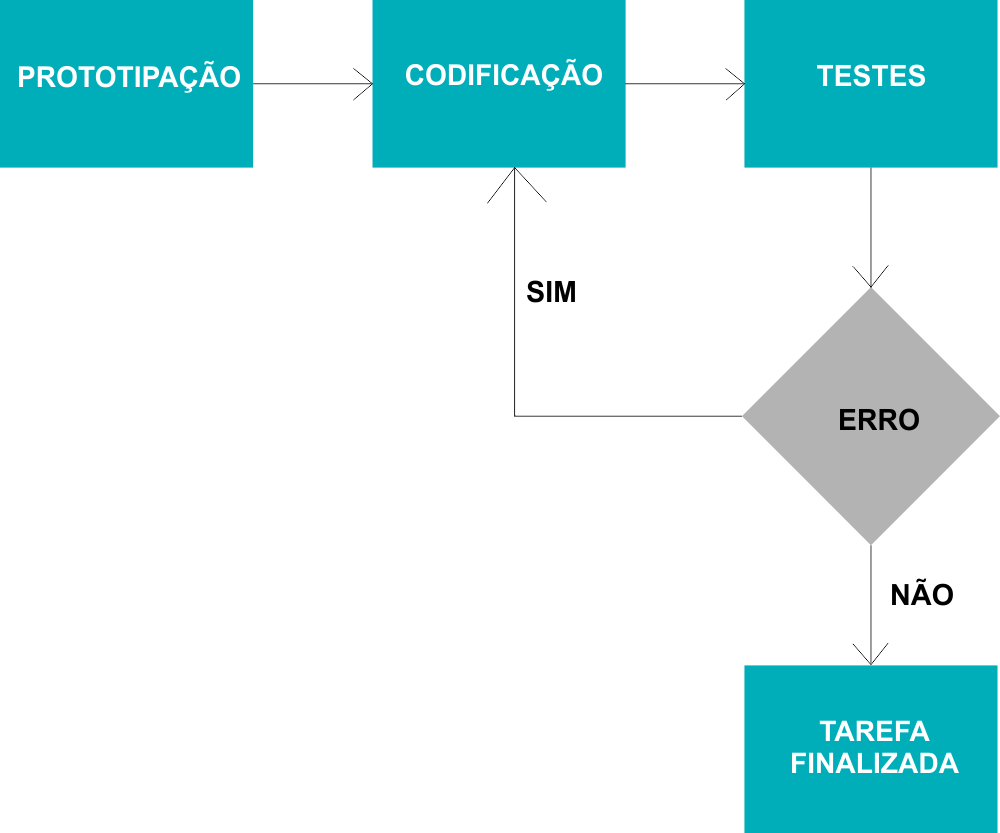
\includegraphics[scale=1]{Figuras/fluxo.png}
  \caption{Fluxo do desenvolvimento do AlfaGebra}
  \label{fluxograma}
\end{figure}

\subsection{Métodos}
\noindent Nesta seção são demonstrados os métodos a serem aplicados para o desenvolvimento da plataforma de ensino e aprendizagem AlfaGebra, com objetivo de explanar detalhadamente como ocorrerão as etapas de prototipagem das telas, aplicação da metodologia de desenvolvimento ágil \textit{Scrum} e teste de usabilidade.

\subsubsection{Prototipagem - Desenho das telas}
\noindent Para a realização da prototipagem das telas, serão desenhadas à mão, ou com \textit{software} específicos para gerar os esboços das telas e uma vez os desenhos concretizados irá oferecer suporte para os programadores no decorrer do desenvolvimento. 

\subsubsection{Desenvolvimento Ágil (\textit{Scrum})}
\noindent Com a aplicação da metodologia de desenvolvimento ágil \textit{Scrum} será possível organizar todas as tarefas de programação da plataforma AlfaGebra, de forma a ter um desenvolvimento intuitivo e organizado. Para a aplicação desta metodologia será utilizada a ferramenta de gerenciamento de projetos colaborativa, Trello\footnote[9]{Trello \url{https://trello.com}}, em virtude da mesma apresentar características como, por exemplo, de ser ajustada de acordo com as necessidades dos usuários.

Para esse projeto a estrutura de representação das tarefas serão divididas em 4 (quatro) colunas, sendo as tarefas a fazer, em desenvolvimento, finalizadas e em testes. Na coluna de tarefas a fazer serão descritas todas as tarefas que serão realizadas para a conclusão do projeto. Na tarefa em desenvolvimento são descritas todas as tarefas que foram inciadas a implementação, mas que ainda não foram concluídas, na finalizada são descritas todas as tarefas que que foram finalizadas e por fim, a coluna em testes são as tarefas que foram finalizadas, mas que estão em teste para verificar alguma falha no seu funcionamento. 

Diante das informações supracitadas todas as tarefas serão baseadas na metodologia de desenvolvimento ágil \textit{Scrum}, a partir do conceito dos \textit{backlog} e das demandas a serem entregas a partir das definições dos \textit{sprints} e o acompanhamento do projeto será realizado periodicamente em reuniões com a equipe do projeto.

\subsubsection{Teste de Usabilidade}
\noindent Em virtude da avaliação do resultado final do \textit{software}, no presente trabalho será aplicado o teste de usabilidade a fim de identificar a performance alcançada pelos usuários e o entendimento das funções do sistema. Visto que uma interface com boa usabilidade possibilita que o usuário torne-se mais produtivo, em virtude em que ele não irá interromper o processo para buscar orientação quanto alguma dúvida do sistema.

Para a concretização do teste será aplicado um questionário, que abrangerá afirmativas com as possibilidades de excelente, ótimo, bom, regular e péssima, junto aos alunos da disciplina de Álgebra Linear do curso de Ciência da Computação que utilizaram o sistema no decorrer do semestre 2017-2 e assim identificar pontos positivos e negativos do sistema e buscar solucionar os negativos em atualizações futuras. 

\begin{comment}
\subsection{Diagramas UML}
\noindent

\subsubsection{Diagrama de Caso de Uso}
\noindent

\subsubsection{Diagrama de Classe}
\noindent

\subsubsection{Diagrama de Atividade}
\noindent

\subsubsection{Diagrama de Implementação}
\noindent
\end{comment}

\subsection{Ferramentas e Materiais}
\noindent Nesta seção são descritas as ferramentas tecnológicas utilizadas para a construção da plataforma de ensino e aprendizagem AlfaGebra. A seguir estão descritos todos os recursos tecnológicos que serão aplicados para que a plataforma possa ser concretizada.

\begin{itemize}
    \item \textit{Plataforma Java Standard Edition} (Java SE)\footnote[10]{Java SE \url{http://www.oracle.com/technetwork/java/javase/overview/index.html}}
\end{itemize}
\noindent A presente plataforma é uma ferramenta para desenvolvimento de \textit{software}, que permite desenvolver e implementar aplicativos Java em \textit{desktops} e servidores. a Java SE é mantida pela empresa Sun Oracle para a comunidade de programadores Java.

\begin{itemize}
    \item JavaFX \textit{Sciene Builder}\footnote[11]{JavaFX \url{http://www.oracle.com/technetwork/pt/java/javafx/overview/index.html}}
\end{itemize}
\noindent JavaFX é uma conjunto de pacotes gráficos e de mídia que possibilita aos programadores criar, testar, depurar e implementar aplicações. Lançada pela a Sun Oracle para a criação de aplicativos para diversas plataformas como \textit{desktop}, web, \textit{mobile}, etc., ela conta com recursos para personalizar a aparência das aplicações, tais como folha de estilos em cascata (CSS), recursos bastante utilizados em desenvolvimento web para personalizar a aparência das aplicações. A escolha dessa biblioteca foi devido às informações supracitadas e que o objetivo é desenvolver uma plataforma com \textit{interface} bem agradável para o usuário.

\begin{itemize}
    \item Netbeans IDE\footnote[12]{Netbeans \url{https://netbeans.org/}}
\end{itemize}
A IDE utilizada para o desenvolvimento do \textit{software} em versão para \textit{desktop} será Netbeans, que oferece suporte de primeira classe para as tecnologias e melhorias de especificações Java mais recentes. Sua escolha foi realizada pela a equipe de desenvolvimento devido a mesma apresentar amplo suporte à criação de aplicações Java e por ser gratuita.

\begin{itemize}
    \item PrimeFaces\footnote[13]{PrimeFaces \url{https://www.primefaces.org/}}
\end{itemize}
Primefaces é um \textit{framework} \textit{openSource} de componentes para Java, que apresenta como objetivo fornecer componentes padrões para \textit{Java Server Faces}. Apesar de sua aplicação ser voltada para desenvolvimento web este estará sendo utilizado para desenvolvimento \textit{desktop}. A escolha dessa ferramenta foi realizada para a geração de gráficos, em virtude da plataforma AlfaGebra irá apresentar, sempre que possível, a interpretação geométrica, de forma a dinamizar, simplificar e otimizar o conhecimento.

\begin{itemize}
    \item iText\footnote[14]{iText \url{https://itextpdf.com}}
\end{itemize}
O iText é um conjunto de ferramentas \textit{open source} desenvolvido para a comunidade de desenvolvedores de \textit{software}, que permite a integração de funcionalidades em PDF \textit{Portable Document Format} (Formato Portátil de Documento) nas aplicações. A sua escolha foi aplicada devido a necessidade de gerar arquivos PDF na plataforma para que os acadêmicos possam ter esse recurso a sua disposição, por exemplo, na resolução de uma determinada questão.

É provável que alguns itens apresentados nesse projeto venham a sofrer alterações no decorrer da execução do desenvolvimento da plataforma, pois na medida que é iniciado o estudo e desenvolvimento, melhores ferramentas podem ser adotas para facilitar o processo.